\documentclass[journal]{IEEEtran}
\usepackage[T1]{fontenc}
\usepackage{cite}
\usepackage{amsmath,amssymb,amsfonts}
\usepackage{graphicx}
\usepackage{textcomp}
\usepackage{booktabs}
\usepackage{array}
\usepackage{tikz}
\usetikzlibrary{positioning,arrows.meta}
\usepackage{algorithm}
\usepackage{algpseudocode}
\usepackage{url}
\hyphenation{op-tical net-works semi-conduc-tor IEEE-Xplore}

\begin{document}

\title{From Data Scarcity to Abundance? A Reproducible Benchmark of Quality-Gated Synthetic Data Pipelines for Tabular Model Training}

\author{Bhavin~Kotak%
\thanks{B. Kotak is with IBM, Armonk, NY, USA (e-mail: bhavin.kotak@ibm.com; ORCID: 0009-0006-4793-7046).}%
\thanks{This is version 2.0 of a preprint first released in January 2026. Version 2.0 replaces the unmeasured claims of version 1 with a preregistered, reproducible benchmark.}%
}

\markboth{Preprint, version 2.0}%
{Kotak: Quality-Gated Synthetic Data Pipelines for Tabular Model Training}

\maketitle

\begin{abstract}
Synthetic data is often proposed for training models when real records are scarce or sensitive. Version 1 of this paper made quantitative claims about such pipelines with no experiment behind them, and this revision replaces those claims with a preregistered, reproducible benchmark. We describe a pipeline in which a planner chooses among candidate generators and a quality gate accepts a synthetic batch only if it stays close to a real holdout and is not closer to training records than fresh real records are. No language-model API was available. The planner is therefore a deterministic rule-based stand-in, and the language-model layer is still an untested design. We evaluate four local generators (Gaussian copula, class-conditional Gaussian mixture, SMOTE-style interpolation, independent marginals) and a memorising control on four public tabular datasets with five seeds. The gated pipeline retained between 96.1\% and 99.6\% of real-data test AUC. That supports the preregistered hypothesis of at least 90\% retention, with no margin on credit-g, where the interval reached the threshold. Utility alone did not reveal leakage. Interpolation and copying kept near-real utility while membership-inference AUC rose as high as 0.82. The gate withheld every interpolation and copy release, and when the copier was tried first it lowered attack AUC to between 0.50 and 0.55. Under a simulated 30\% fault rate, retry with fallback delivered 99.5\% of requested rows (53420 of 53920). Adding synthetic rows to small real training sets gave no consistent gain.
\end{abstract}

\begin{IEEEkeywords}
Synthetic data, tabular data, data quality gate, membership inference, privacy evaluation, machine learning pipelines, preregistration, reproducibility
\end{IEEEkeywords}

\IEEEpeerreviewmaketitle

\section{Introduction}
\label{sec:intro}

\IEEEPARstart{S}{ynthetic} data generation fits a model to real records and samples new records from it. Teams use it to share data across organisational boundaries, to augment small training sets, and to test pipelines without access to production records~\cite{jordon2022synthetic,chen2021synthetic,hernandez2022synthetic}. Large language models (LLMs) add one more option. They can generate records directly or coordinate other generators~\cite{borisov2023great,long2024llm}.

Version~1 of this paper proposed an LLM-orchestrated pipeline for this setting. It reported that models trained on synthetic data reached a fixed share of real-data performance, that costs and development time fell sharply, and that privacy risk disappeared. None of these figures came from an experiment. The case studies had no data behind them and several numbers had no source, so a reader could neither reproduce nor falsify them.

This revision keeps the architectural idea and drops every number that was not measured. It asks three questions, all of which can be answered on public data with a laptop CPU. How much downstream utility does a gated pipeline of simple, locally fitted generators retain on standard tabular tasks? Does a quality gate change what is released, and can utility alone detect privacy leakage? And how does the pipeline behave at its breakpoints, that is, with small real samples, missing values, and failing generators?

We preregistered the hypothesis, the primary endpoint, and the decision rule before running any experiment (Section~\ref{sec:eval}). The paper contributes the following.
\begin{itemize}
\item A pipeline architecture with a planner, a generator pool, schema validation, a fail-closed quality gate, and an explicit abstention rule, whose gate thresholds are calibrated against real-versus-real batches of equal size (Section~\ref{sec:method}).
\item A benchmark of four generators and a memorising control on four public datasets, with utility, fidelity, and privacy measured on disjoint splits over five seeds.
\item Evidence that utility ratios are a weak signal: a generator that copies training rows keeps near-real utility, yet a simple membership attack against it succeeds well above chance.
\item Breakpoint scenarios for data scarcity, missing data, and simulated generator faults, each reported with intervals and with the ablations that attribute the effect.
\end{itemize}
We do not evaluate the LLM planner itself. Section~\ref{sec:threats} records this and the other untested assumptions.

\section{Related Work}
\label{sec:related}

\subsection{Tabular data generators}
Deep generative models for tables include GAN-based designs~\cite{goodfellow2014gan} such as CTGAN~\cite{xu2019ctgan} and CTAB-GAN~\cite{zhao2021ctabgan}, and diffusion models such as TabDDPM~\cite{kotelnikov2023tabddpm}. The Synthetic Data Vault popularised Gaussian-copula models for relational data~\cite{patki2016sdv}. PrivBayes releases data through a differentially private Bayesian network~\cite{zhang2017privbayes}. SMOTE creates minority-class records by interpolating between neighbours~\cite{chawla2002smote}. It was designed to oversample a training set, and releasing its output is a different use. We include it because interpolation is a common shortcut in practice. Language models can also generate rows when a table is serialised as text~\cite{borisov2023great}. Reviews in health care survey these families and their evaluation~\cite{hernandez2022synthetic,chen2021synthetic}. Our study is limited to generators that fit in seconds on a CPU, so deep generators are an unavailable baseline (Section~\ref{sec:threats}).

\subsection{LLM-driven synthetic data}
Self-Instruct showed that a language model can bootstrap its own training data from a small seed set~\cite{wang2023selfinstruct}. A recent survey organises LLM-driven generation into generation, curation, and evaluation stages~\cite{long2024llm}. Our architecture uses the same split: the planner proposes, the gate curates, and the evaluation harness measures. Only the parts that need no LLM are measured here.

\subsection{Evaluating synthetic data}
Train-on-synthetic, test-on-real (TSTR) evaluation was introduced for medical time series~\cite{esteban2017rcgan} and is now the standard utility test. Sample-level fidelity, diversity, and authenticity metrics were proposed to audit generative models~\cite{alaa2022faithful}. Holdout-based distance-to-closest-record tests compare synthetic records with a real holdout instead of an absolute threshold~\cite{platzer2021holdout}, and our privacy rule follows that design. Benchmarking libraries such as Synthcity bundle many of these metrics~\cite{qian2023synthcity}. Van Breugel et al. warn that errors in the generator propagate to every downstream analysis~\cite{vanbreugel2023synthetic}. Tree ensembles remain strong on tabular data~\cite{grinsztajn2022tree}, so a gradient-boosted classifier is our primary downstream model.

\subsection{Privacy of synthetic data}
Differential privacy gives formal guarantees~\cite{dwork2006calibrating}, but most deployed generators are not differentially private. Membership inference attacks test whether a record was in the training set~\cite{shokri2017membership}. Attacks against generative models use either a discriminator~\cite{hayes2017logan} or Monte Carlo distance estimates~\cite{hilprecht2019monte}. TAPAS packages several attacks for auditing~\cite{houssiau2022tapas}. We use a distance-based attack because it is simple and transparent; a stronger attack would only raise the leakage we report.

\subsection{Data validation in pipelines}
Declarative data-quality checks that block bad batches are an established pattern in production machine learning~\cite{schelter2018automating}. Our gate applies the same idea to synthetic batches. Its thresholds come from real data. None is set by hand.

\section{Methodology}
\label{sec:method}

\subsection{System model}
A real dataset $\mathcal{D}=\{(x_i,y_i)\}_{i=1}^{N}$ has $d$ feature columns, each numeric or categorical, and a binary label $y_i\in\{0,1\}$. For each seed we draw a stratified split into a train set $\mathcal{D}_{\mathrm{tr}}$ (half of the rows), a holdout $\mathcal{D}_{\mathrm{ho}}$, and a test set $\mathcal{D}_{\mathrm{te}}$ (a quarter each). Generators see only $\mathcal{D}_{\mathrm{tr}}$, the gate and the privacy metrics use $\mathcal{D}_{\mathrm{ho}}$, and utility is measured on $\mathcal{D}_{\mathrm{te}}$ alone. A request asks for $n=|\mathcal{D}_{\mathrm{tr}}|$ synthetic rows, delivered in $K$ batches of size $b=\lceil n/K\rceil$.

Fig.~\ref{fig:arch} shows the architecture. A planner orders the candidate generators, and each call returns a batch that goes through schema validation and then the quality gate. A rejected batch triggers a retry or a fallback to the next candidate. If too few rows pass, the pipeline abstains and releases nothing.

\begin{figure}[!t]
\centering
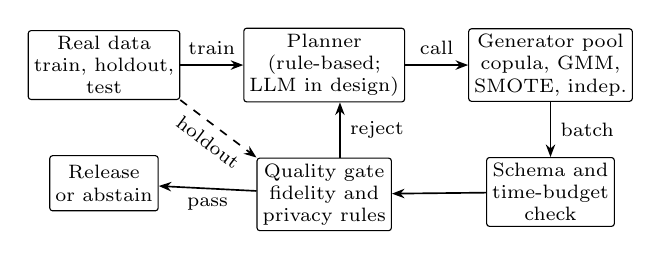
\begin{tikzpicture}[font=\scriptsize, node distance=7mm and 8mm,
  box/.style={draw, rounded corners=1pt, align=center, minimum height=7mm, inner sep=2pt},
  arr/.style={-{Stealth[length=1.6mm]}, semithick}]
\node[box] (real) {Real data\\ train, holdout,\\ test};
\node[box, right=of real] (plan) {Planner\\ (rule-based;\\ LLM in design)};
\node[box, right=of plan] (pool) {Generator pool\\ copula, GMM,\\ SMOTE, indep.};
\node[box, below=of pool] (val) {Schema and\\ time-budget\\ check};
\node[box, below=of plan] (gate) {Quality gate\\ fidelity and\\ privacy rules};
\node[box, below=of real] (rel) {Release\\ or abstain};
\draw[arr] (real) -- node[above]{train} (plan);
\draw[arr] (plan) -- node[above]{call} (pool);
\draw[arr] (pool) -- node[right]{batch} (val);
\draw[arr] (val) -- (gate);
\draw[arr] (gate) -- node[below]{pass} (rel);
\draw[arr] ([xshift=2mm]gate.north) -- node[right]{reject} ([xshift=2mm]plan.south);
\draw[arr, dashed] (real.south east) -- node[pos=0.5, below, sloped]{holdout} (gate.north west);
\end{tikzpicture}
\caption{Pipeline architecture. The planner orders the candidate generators, and every batch goes through schema validation and a quality gate calibrated on the real holdout. A rejection triggers a retry or a fallback. The dashed arrow is the holdout used for gate calibration and privacy tests.}
\label{fig:arch}
\end{figure}

\subsection{Generators}
All generators are class-conditional. They fit one model per label value and sample labels with the training class prior. Each column is mapped to a numeric code (categories are coded by descending frequency), and a randomised probability integral transform turns the codes into normal scores; ties are spread uniformly inside their jump of the empirical CDF.

\emph{Gaussian copula.} Let $F_{j\mid y}$ be the empirical CDF of column $j$ in class $y$ and $\Phi$ the standard normal CDF. Let $R_y$ be the Ledoit-Wolf shrunk correlation matrix of the normal scores in class $y$. A record is drawn as
\begin{equation}
z\sim\mathcal{N}(0,R_y),\qquad x_j=F_{j\mid y}^{-1}\bigl(\Phi(z_j)\bigr),\quad j=1,\dots,d.
\label{eq:copula}
\end{equation}
For numeric columns with at least 20 distinct values, $F^{-1}$ interpolates between order statistics. Other columns use the inverted CDF, so every sampled category exists in the training data.

\emph{Class-conditional GMM.} A Gaussian mixture with full covariance replaces $\mathcal{N}(0,R_y)$ in \eqref{eq:copula}. BIC selects the number of components from $\{1,2,4,8\}$, with at least 10 rows per component and covariance regularisation 0.001.

\emph{SMOTE-style interpolation.} Take a random training record $x_a$ and one of its $k=5$ nearest same-class neighbours $x_c$ under the Gower distance $g$ of \eqref{eq:dcr}. Numeric columns are set to
\begin{equation}
x=x_a+\lambda\,(x_c-x_a),\qquad \lambda\sim\mathcal{U}(0,1).
\label{eq:smote}
\end{equation}
Integer columns are rounded. Categorical columns take the value of $x_a$ when $\lambda<0.5$ and of $x_c$ otherwise.

\emph{Independent marginals.} This is the copula with $R_y=I$. It keeps every class-conditional marginal and discards dependence, so it is the floor a useful generator must beat.

\emph{Leaky copy (control).} This generator resamples training records verbatim. It is never a candidate in the orchestrated pipeline; it is there to test whether the metrics and the gate detect memorisation.

\subsection{Metrics}
Let $f_{\mathcal{S}}$ be a classifier trained on a set $\mathcal{S}$ and $\mathrm{AUC}(f;\mathcal{D}_{\mathrm{te}})$ its ROC-AUC on the test split. The utility ratio of a synthetic set $\mathcal{S}$ is
\begin{equation}
U(\mathcal{S})=\frac{\mathrm{AUC}(f_{\mathcal{S}};\mathcal{D}_{\mathrm{te}})}{\mathrm{AUC}(f_{\mathcal{D}_{\mathrm{tr}}};\mathcal{D}_{\mathrm{te}})}.
\label{eq:utility}
\end{equation}
The numerator is TSTR; the denominator is train-on-real, test-on-real (TRTR) with the same classifier and seed.

For two tables $A$ and $B$, the marginal distance averages a per-column distance $\delta_j$. On a numeric column, $\delta_j$ is the two-sample Kolmogorov-Smirnov statistic; on a categorical column it is the total-variation distance between the category frequencies $\hat p_{A,j}$ and $\hat p_{B,j}$:
\begin{equation}
M(A,B)=\frac{1}{d}\sum_{j=1}^{d}\delta_j,\qquad \delta_j^{\mathrm{cat}}=\frac{1}{2}\sum_{v}\bigl|\hat p_{A,j}(v)-\hat p_{B,j}(v)\bigr|.
\label{eq:marginal}
\end{equation}
The correlation distance compares Spearman coefficients $\rho_{jk}$ computed on the column codes:
\begin{equation}
C(A,B)=\frac{2}{d(d-1)}\sum_{j<k}\bigl|\rho_{jk}(A)-\rho_{jk}(B)\bigr|.
\label{eq:corr}
\end{equation}

For privacy, let $r_j$ be the range of numeric column $j$ in the train split, and let the label count as one more categorical column. The Gower distance $g$ and the distance-to-closest-record (DCR) share $P$ are
\begin{equation}
\begin{split}
g(a,c)&=\sum_{j\in\mathrm{num}}\frac{|a_j-c_j|}{r_j}+\sum_{j\in\mathrm{cat}}\mathbf{1}[a_j\neq c_j],\\
P(\mathcal{S})&=\frac{1}{|\mathcal{S}|}\sum_{s\in\mathcal{S}}\Bigl(\mathbf{1}[d_T(s)<d_H(s)]+\tfrac{1}{2}\mathbf{1}[d_T(s)=d_H(s)]\Bigr).
\end{split}
\label{eq:dcr}
\end{equation}
Here $d_T(s)$ and $d_H(s)$ are the distances from $s$ to its nearest record in a random train subsample $T$ and in the holdout $H$, with $|T|=|H|$. A generator that is no closer to its training data than to fresh data gives $P\approx 0.5$, and a copier gives values well above it~\cite{platzer2021holdout}. For evaluation, $\mathcal{S}$ is subsampled to at most 2000 records.

The membership attack scores a candidate record $x$ by $a(x)=-\min_{s\in\mathcal{S}}g(x,s)$. Members are the records in $T$; non-members are those in $H$. The attack AUC is
\begin{equation}
\mathrm{MIA}(\mathcal{S})=\Pr\bigl[a(x_T)>a(x_H)\bigr]+\tfrac{1}{2}\Pr\bigl[a(x_T)=a(x_H)\bigr],
\label{eq:mia}
\end{equation}
with $x_T$ drawn from $T$ and $x_H$ from $H$. Chance level is 0.5. We also report the exact-match rate, the fraction of synthetic records at distance zero from $T$.

\subsection{Quality gate}
Thresholds on $M$ and $C$ depend on sample size, column types, and the dataset, so the fixed cut-offs used in version~1 do not transfer. We calibrate them per dataset and seed instead: draw $R=20$ random batches of $b$ real training rows and compute $M$ and $C$ against the holdout. Let $q_{0.95}(\cdot)$ denote the empirical 0.95 quantile over these draws. A batch $B$ is accepted when
\begin{equation}
\begin{split}
\gamma(B)=\;&\mathbf{1}\bigl[M(B,\mathcal{D}_{\mathrm{ho}})\le\kappa\,q_{0.95}(M_{\mathrm{ref}})\bigr]\\
\cdot\;&\mathbf{1}\bigl[C(B,\mathcal{D}_{\mathrm{ho}})\le\kappa\,q_{0.95}(C_{\mathrm{ref}})\bigr]\cdot\mathbf{1}\bigl[P(B)\le\tau\bigr]=1,
\end{split}
\label{eq:gate}
\end{equation}
with preregistered values $\kappa=2$ and $\tau=0.6$. The fidelity rules ask that a synthetic batch look no worse than twice the high-end sampling noise of real batches. The privacy rule asks that it not be much closer to training records than to fresh ones.

\subsection{Orchestration objective}
The planner receives an ordered candidate list $\mathcal{G}=(G_1,\dots,G_m)$. Let $\mathcal{B}$ be the set of accepted batches and $\mathcal{S}=\bigcup_{B\in\mathcal{B}}B$ the release. The pipeline seeks
\begin{equation}
\begin{split}
\max_{\mathcal{S}}\;&U(\mathcal{S})\\
\text{s.t.}\;&\gamma(B)=1\ \ \forall B\in\mathcal{B},\quad |\mathcal{S}|\ge\alpha n,\quad c\le A\,m,
\end{split}
\label{eq:objective}
\end{equation}
where $c$ counts the generator calls spent on one batch slot, $A$ is the attempt limit per candidate, and $\alpha$ is the minimum release fraction. If the size constraint fails, the pipeline abstains. The pipeline cannot see the test split, so it cannot measure utility while it generates. Instead the planner uses a fixed order as a proxy for expected utility, going from the most to the least structure-preserving generator: copula, GMM, SMOTE-style, then independent marginals. Algorithm~\ref{alg:orch} solves \eqref{eq:objective} greedily, one batch slot at a time, with the preregistered settings $K=10$, $A=2$, and $\alpha=0.5$.

\begin{algorithm}[!t]
\caption{Gated orchestration of one synthetic-data request}
\label{alg:orch}
\begin{algorithmic}[1]
\small
\Require candidates $(G_1,\dots,G_m)$, rows $n$, batches $K$, attempts $A$, release fraction $\alpha$, time budget $t_{\max}$
\State $b\gets\lceil n/K\rceil$; $\mathcal{S}\gets\emptyset$
\For{slot $=1,\dots,K$}
  \For{$G$ in $(G_1,\dots,G_m)$, up to $A$ calls each}
    \State call $G$ for $b$ rows; on exception log \textsc{error}
    \State if elapsed time $>t_{\max}$, log \textsc{timeout}
    \State if schema is violated or values are missing, log \textsc{invalid}
    \State evaluate \eqref{eq:gate}; if a metric is undefined, log \textsc{unknown}
    \If{$\gamma(B)=1$}
      \State $\mathcal{S}\gets\mathcal{S}\cup B$; go to the next slot
    \EndIf
  \EndFor
\EndFor
\State \Return $\mathcal{S}$ if $|\mathcal{S}|\ge\alpha n$, else \textsc{abstain}
\end{algorithmic}
\end{algorithm}

\subsection{Outcome handling}
Every external call has a defined outcome. A generator exception counts as a failed call and triggers a retry or a fallback. A call that runs past the 30-second time budget is discarded as a timeout, and a batch with the wrong columns, the wrong length, or missing values is rejected as invalid. The gate fails closed: if a gate metric is undefined, for example because a column is empty, the batch is rejected. Missing values in the real data are handled before fitting. Inside the generators a missing category becomes its own level and a missing numeric cell gets the training median. Utility can be missing too, when a training set holds a single class; we record it as missing and never impute it. A run that abstains contributes no utility or privacy value. Abstentions are reported as counts.

\subsection{Role of the language model}
In the intended design, an LLM would replace the fixed candidate order. It would read the schema and the gate log, propose generator settings or constraints, and explain rejections. Everything it produced would still go through the same gate, which therefore bounds what any planner can release. We had no LLM API and do not measure this layer. The rule-based planner is only a lower baseline for it.

\section{Evaluation}
\label{sec:eval}

\subsection{Setup}
\emph{Preregistration.} The hypothesis, endpoints, thresholds, and decision rule went into \texttt{preregistration.json} before the runs. Hypothesis H1 states that the gated, orchestrated pipeline retains at least 90\% of real-data utility on each dataset while its synthetic records are no closer to training records than fresh records are. The primary endpoint is the HGB utility ratio \eqref{eq:utility}, averaged over five seeds with a two-sided 95\% Student-t interval. H1 is SUPPORTED if, on every dataset, the lower interval bound is at least 0.9, the mean DCR share is at most 0.6, and no seed abstains. It is REFUTED if any upper bound falls below 0.9, if any DCR interval lies above 0.6, or if the pipeline abstains in at least 3 of 5 seeds on a dataset. Otherwise it is INCONCLUSIVE. We also preregistered secondary endpoints for gate attribution (S1), scarcity (S2), and fault tolerance (S3); missing-data injection and runtime scaling are exploratory.

\emph{Data.} Table~\ref{tab:datasets} lists the four public binary classification datasets: Wisconsin diagnostic breast cancer~\cite{street1993nuclear}, German credit~\cite{hofmann1994statlog}, Adult census income~\cite{becker1996adult}, and bank marketing~\cite{moro2014bank}. The last three were retrieved from OpenML~\cite{vanschoren2014openml}; the first ships with scikit-learn~\cite{pedregosa2011scikit}. To bound runtime, any dataset with more than 10000 rows is subsampled per seed to 10000 rows, stratified by label.

% AUTO:BEGIN datasets
\begin{table}[!t]
\caption{Benchmark datasets (public, binary classification). Rows used per seed after the stratified cap of 10000 rows.}
\label{tab:datasets}
\centering
\footnotesize
\setlength{\tabcolsep}{3pt}
\begin{tabular}{lrrrrr}
\toprule
Dataset & Rows & Num. & Cat. & Pos. rate & Rows used \\
\midrule
Breast cancer & 569 & 30 & 0 & 0.373 & 569 \\
Credit-g & 1000 & 7 & 13 & 0.300 & 1000 \\
Adult & 48842 & 6 & 8 & 0.239 & 10000 \\
Bank marketing & 45211 & 7 & 9 & 0.117 & 10000 \\
\bottomrule
\end{tabular}
\end{table}
% AUTO:END datasets

\emph{Classifiers.} The primary downstream model is a histogram gradient-boosted tree ensemble (HGB) with 200 iterations and default settings otherwise. The second is a logistic regression (LR) with median imputation, standardisation, and one-hot encoding. Both come from scikit-learn~\cite{pedregosa2011scikit}, and one seed drives the split, the generators, and the models.

\emph{Conditions.} For each dataset and seed we evaluate every generator without the gate (ungated) and every generator as the only candidate behind the gate (gated). We also run the orchestrated pipeline and an adversarial order that places the leaky copy first. Two references bound the metrics: TRTR for utility, and the real test split itself (``fresh real'') for fidelity and privacy.

\emph{Breakpoints.} Scenario E2 (scarcity) fits the generators on $n_{\mathrm{real}}\in\{50,100,200,400\}$ stratified training rows; the gate then uses a holdout of the same size, and the pipeline requests 4 synthetic rows per real row. Real-only, synthetic-only, and real-plus-synthetic training are compared on the full test split. Breast cancer has fewer than 400 training rows, so we skip its largest setting. Scenario E3 (missing data) deletes 10\% or 30\% of the numeric cells in the train and holdout splits completely at random. In Scenario E4 (faults), every candidate is wrapped so that each call fails with probability $p\in\{0,0.1,0.3,0.5\}$. Failures are split equally between an exception, a timeout, and a corrupt batch, and E4 compares retry with fallback against one attempt on one candidate. Scenario E5 times fitting, sampling, gating, and privacy evaluation on Adult.

\emph{Environment.} All runs used one Apple-silicon laptop with 8 CPU cores, Python 3.12, and scikit-learn 1.9.1. From cached data to figures, the full experiment took 470 seconds of wall-clock time. Every number below is read from the \texttt{results/} files that this run writes.

\subsection{Results}

\subsubsection{Primary endpoint}
Fig.~\ref{fig:utility} and Table~\ref{tab:utility} report the utility ratios. The orchestrated, gated pipeline reached mean HGB ratios of 0.996 on breast cancer, 0.961 on credit-g, 0.990 on Adult, and 0.962 on bank marketing, with 95\% intervals of $[0.982, 1.009]$, $[0.900, 1.023]$, $[0.986, 0.995]$, and $[0.931, 0.994]$. Mean DCR shares were 0.527, 0.502, 0.497, and 0.508. No run abstained. Under the preregistered rule the verdict is SUPPORTED, but the margin on credit-g is negligible: its lower bound equals the threshold to three decimals, and a sixth seed could move it either way. Credit-g also has the lowest TRTR AUC (0.762), so it carries most of the uncertainty.

\begin{figure}[!t]
\centering
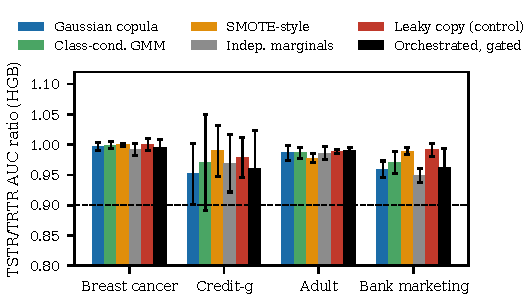
\includegraphics[width=\columnwidth]{figures/utility_ratio.pdf}
\caption{Utility ratio TSTR/TRTR with the HGB classifier (mean and 95\% interval over five seeds) for ungated generators and the gated, orchestrated pipeline. Dashed line: the preregistered target of 0.9.}
\label{fig:utility}
\end{figure}

% AUTO:BEGIN utility
\begin{table*}[!t]
\caption{Utility ratio TSTR/TRTR (ROC-AUC on the real test split) for the HistGradientBoosting (HGB) and logistic-regression (LR) classifiers, mean over five seeds. Gated rows average only the runs in which data were released (see Table~\ref{tab:gate}); SMOTE-style and leaky-copy gated runs never released data on any dataset and are omitted.}
\label{tab:utility}
\centering
\scriptsize
\setlength{\tabcolsep}{2.5pt}
\begin{tabular}{lw{c}{20pt}w{c}{20pt}w{c}{20pt}w{c}{20pt}w{c}{20pt}w{c}{20pt}w{c}{20pt}w{c}{20pt}}
\toprule
Condition & \multicolumn{2}{c}{Breast cancer} & \multicolumn{2}{c}{Credit-g} & \multicolumn{2}{c}{Adult} & \multicolumn{2}{c}{Bank marketing} \\
 & HGB & LR & HGB & LR & HGB & LR & HGB & LR \\
\midrule
Gaussian copula, ungated & 0.997 & 0.997 & 0.952 & 0.987 & 0.987 & 0.990 & 0.960 & 0.975 \\
Class-cond.\ GMM, ungated & 0.999 & 0.998 & 0.970 & 0.998 & 0.986 & 0.989 & 0.970 & 0.977 \\
SMOTE-style, ungated & 1.000 & 1.001 & 0.990 & 0.967 & 0.977 & 0.995 & 0.989 & 0.996 \\
Indep.\ marginals, ungated & 0.992 & 0.988 & 0.970 & 0.979 & 0.986 & 0.988 & 0.949 & 0.960 \\
Leaky copy (control), ungated & 1.000 & 1.002 & 0.978 & 0.980 & 0.989 & 0.997 & 0.991 & 0.993 \\
Gaussian copula, gated & 0.996 & 0.999 & 0.960 & 0.991 & 0.986 & 0.991 & 0.956 & 0.974 \\
Class-cond.\ GMM, gated & 0.998 & 0.997 & 0.969 & 0.983 & 0.985 & 0.989 & 0.969 & 0.974 \\
Indep.\ marginals, gated & 0.991 & 0.990 & 0.985 & 0.979 & 0.986 & 0.989 & n/a & n/a \\
Orchestrated, gated & 0.996 & 1.000 & 0.961 & 0.965 & 0.990 & 0.991 & 0.962 & 0.975 \\
Adversarial order, gated & 0.994 & 0.998 & 0.960 & 0.986 & 0.986 & 0.991 & 0.965 & 0.980 \\
\bottomrule
\end{tabular}
\end{table*}
% AUTO:END utility

% AUTO:BEGIN privacy
\begin{table*}[!t]
\caption{Fidelity and privacy, mean over five seeds. Marg.: mean per-column KS/TV distance to the holdout. Corr.: mean absolute Spearman-correlation difference. DCR: share of synthetic records nearer to training records than to holdout records (0.5 is the fresh-real reference). MIA: AUC of the distance-based membership attack (0.5 is chance).}
\label{tab:privacy}
\centering
\scriptsize
\setlength{\tabcolsep}{2.5pt}
\begin{tabular}{lcccccccccccccccc}
\toprule
Condition & \multicolumn{4}{c}{Breast cancer} & \multicolumn{4}{c}{Credit-g} & \multicolumn{4}{c}{Adult} & \multicolumn{4}{c}{Bank marketing} \\
 & Marg. & Corr. & DCR & MIA & Marg. & Corr. & DCR & MIA & Marg. & Corr. & DCR & MIA & Marg. & Corr. & DCR & MIA \\
\midrule
Fresh real (reference) & 0.099 & 0.077 & 0.483 & 0.476 & 0.054 & 0.075 & 0.483 & 0.483 & 0.019 & 0.022 & 0.500 & 0.500 & 0.017 & 0.022 & 0.501 & 0.496 \\
Gaussian copula, ungated & 0.101 & 0.074 & 0.550 & 0.505 & 0.049 & 0.080 & 0.523 & 0.491 & 0.019 & 0.056 & 0.507 & 0.503 & 0.018 & 0.056 & 0.511 & 0.499 \\
Class-cond.\ GMM, ungated & 0.106 & 0.074 & 0.551 & 0.513 & 0.049 & 0.078 & 0.531 & 0.496 & 0.024 & 0.052 & 0.497 & 0.502 & 0.021 & 0.044 & 0.505 & 0.500 \\
SMOTE-style, ungated & 0.100 & 0.096 & 0.787 & 0.788 & 0.060 & 0.073 & 0.762 & 0.775 & 0.034 & 0.026 & 0.742 & 0.635 & 0.031 & 0.023 & 0.759 & 0.646 \\
Indep.\ marginals, ungated & 0.097 & 0.218 & 0.480 & 0.500 & 0.051 & 0.094 & 0.512 & 0.493 & 0.018 & 0.067 & 0.497 & 0.503 & 0.016 & 0.084 & 0.500 & 0.497 \\
Leaky copy (control), ungated & 0.098 & 0.071 & 0.741 & 0.799 & 0.048 & 0.070 & 0.735 & 0.820 & 0.019 & 0.023 & 0.760 & 0.672 & 0.017 & 0.022 & 0.746 & 0.664 \\
Orchestrated, gated & 0.098 & 0.088 & 0.527 & 0.509 & 0.047 & 0.078 & 0.502 & 0.498 & 0.019 & 0.055 & 0.497 & 0.504 & 0.018 & 0.056 & 0.508 & 0.497 \\
Adversarial order, gated & 0.104 & 0.081 & 0.556 & 0.550 & 0.047 & 0.080 & 0.542 & 0.521 & 0.019 & 0.056 & 0.508 & 0.502 & 0.018 & 0.057 & 0.505 & 0.501 \\
\bottomrule
\end{tabular}
\end{table*}
% AUTO:END privacy

This result needs qualifying. Every ungated generator, independent marginals included, retained at least 0.949 of TRTR AUC on average, so a class-conditional model that ignores all feature dependence lost little on these tasks. The utility ratio is a lenient test. Passing it says little about whether the joint distribution was learned. The leaky copy reached ratios between 0.979 and 1.000, which means utility cannot tell a useful generator from a memorising one. Nor did the gate change utility. Paired differences between the gated and ungated copula had 95\% intervals that included zero on all four datasets (\texttt{gate\_effect.csv}), and the same held for the orchestrated pipeline against the ungated copula.

\subsubsection{Fidelity and privacy}
Table~\ref{tab:privacy} and Fig.~\ref{fig:privacy} separate the generators that utility could not. For the copula, GMM, and independent-marginals generators, DCR shares fell between 0.480 and 0.551 and attack AUCs \eqref{eq:mia} between 0.491 and 0.513, close to the fresh-real reference. SMOTE-style interpolation looked different. Its DCR shares ran from 0.742 to 0.787 and its attack AUCs from 0.635 to 0.788, because interpolated records \eqref{eq:smote} lie on segments between training neighbours and so sit close to members. The leaky copy produced attack AUCs between 0.664 and 0.820, and about half of its records (0.490 to 0.514) matched a record of the train subsample exactly. On every dataset, independent marginals had the largest correlation distance \eqref{eq:corr}, which is what discarded dependence should look like. Marginal distances \eqref{eq:marginal} stayed near the fresh-real reference for the copula, GMM, and independent generators. SMOTE-style interpolation roughly doubled them on Adult and bank marketing.

\begin{figure}[!t]
\centering
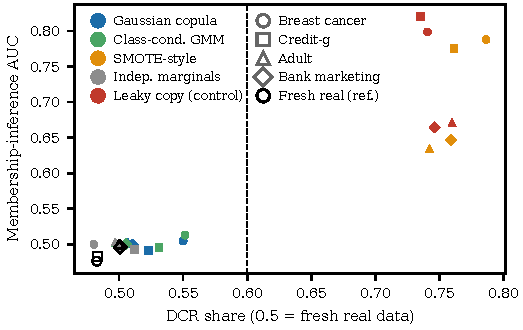
\includegraphics[width=\columnwidth]{figures/privacy.pdf}
\caption{DCR share against membership-inference AUC for ungated generators (filled markers, mean over five seeds) and the fresh-real reference (open markers). Dashed line: the gate threshold of 0.6 on the DCR share.}
\label{fig:privacy}
\end{figure}

\subsubsection{Gate ablation}
Table~\ref{tab:gate} attributes the release decisions to the two gate rules. The privacy rule rejected SMOTE-style batches in all 20 runs, so this generator never released data, and the leaky copy was withheld in all 20 runs as well. On bank marketing, the fidelity rule rejected independent-marginals batches in every seed (94 of 97 calls) because the correlation distance exceeded its threshold. The same generator passed on the other three datasets. The fidelity threshold is calibrated to sampling noise, and on those tables the dependence was weak enough that the independent model stayed within twice that noise.

% AUTO:BEGIN gate
\begin{table}[!t]
\caption{Quality-gate outcomes pooled over four datasets and five seeds. Accept = accepted batches / generator calls. Fid./Priv. = rejections by the fidelity or privacy rule. Abst. = runs (of 20) in which the pipeline withheld release.}
\label{tab:gate}
\centering
\footnotesize
\setlength{\tabcolsep}{2.5pt}
\begin{tabular}{lrrrrr}
\toprule
Condition & Calls & Accept & Fid. & Priv. & Abst. \\
\midrule
Gaussian copula, gated & 215 & 0.916 & 0 & 18 & 0 \\
Class-cond.\ GMM, gated & 215 & 0.916 & 0 & 18 & 0 \\
SMOTE-style, gated & 400 & 0.005 & 0 & 398 & 20 \\
Indep.\ marginals, gated & 265 & 0.558 & 102 & 15 & 5 \\
Leaky copy (control), gated & 397 & 0.018 & 0 & 390 & 20 \\
Orchestrated, gated & 226 & 0.885 & 0 & 26 & 0 \\
Adversarial order, gated & 627 & 0.319 & 0 & 427 & 0 \\
\bottomrule
\end{tabular}
\end{table}
% AUTO:END gate

The adversarial order tests whether the gate protects a pipeline whose first candidate memorises. The copier was tried first for every batch, yet the release consisted mostly of copula batches. Mean attack AUC fell from 0.799 to 0.550 on breast cancer, from 0.820 to 0.521 on credit-g, from 0.672 to 0.502 on Adult, and from 0.664 to 0.501 on bank marketing. The paired reductions in DCR share had 95\% intervals below zero on all four datasets. Protection was incomplete on the two small datasets. With batches of 29 and 50 rows the batch-level DCR share is noisy, and 9 copied batches got through in total, leaving exact-match rates of 0.061 on breast cancer and 0.031 on credit-g. The same noise caused false rejections of genuine batches. The privacy rule rejected 26 orchestrated batches, all of them on the two small datasets. The secondary endpoint S1 (attack AUC at most 0.55 under the adversarial order) was met, though only narrowly on breast cancer.

\subsubsection{Generator faults}
Fig.~\ref{fig:faults} shows the delivered fraction under simulated faults (E4). The failures are simulated; no real API was measured. Each fault rate covers 20 runs (four datasets, five seeds) that together request 53920 rows. With retry and fallback, the pipeline delivered 1.000, 1.000, 0.995, and 0.965 of the requested rows at fault probabilities 0, 0.1, 0.3, and 0.5 (mean of per-run fractions). That is 53420 of 53920 rows at $p=0.3$ and 51791 at $p=0.5$. It never abstained. One attempt on one candidate delivered 0.881, 0.821, 0.615, and 0.506 (35757 of 53920 rows at $p=0.3$) and abstained in 1, 4, and 10 of 20 runs at the three non-zero fault rates. That policy lost rows even without faults, because noisy privacy checks on small batches rejected genuine batches and there was no second chance. The preregistered endpoint S3 (at least 0.95 delivered at $p=0.3$ on every dataset) was met; the lowest dataset mean was 0.980. Delivered batches kept their utility, with the pooled HGB ratio of the retry policy between 0.974 and 0.983 across fault rates.

\begin{figure}[!t]
\centering
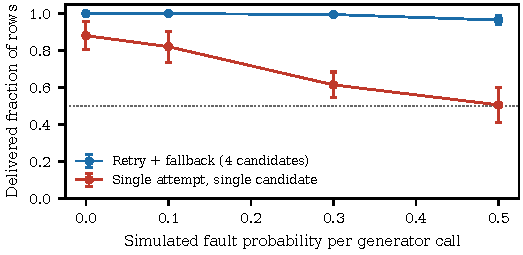
\includegraphics[width=\columnwidth]{figures/faults.pdf}
\caption{Simulated generator faults: fraction of requested rows delivered (mean and 95\% interval over 20 runs). Below the dotted line, the release threshold $\alpha=0.5$, the pipeline abstains.}
\label{fig:faults}
\end{figure}

\subsubsection{Data scarcity}
The title of version~1 promised abundance from scarcity, and Fig.~\ref{fig:scarcity} tests that promise directly (E2). Adding gated synthetic rows to a small real training set did not help consistently. With the LR model at 50 real rows, the paired gain over real-only training was 0.033 on Adult, with interval $[0.010, 0.056]$; on the other three datasets the interval included zero. The HGB model gained on Adult at 200 and 400 rows (0.051 and 0.027, with intervals above zero) and lost 0.027 on bank marketing at 50 rows, with interval $[-0.046, -0.008]$. At 50 rows the gated release abstained in one of five seeds on breast cancer and on Adult, because the noisy privacy rule rejected too many batches. On some tables, synthetic data from these generators can stand in for a small real sample. It does not create information that the sample lacks.

\begin{figure*}[!t]
\centering
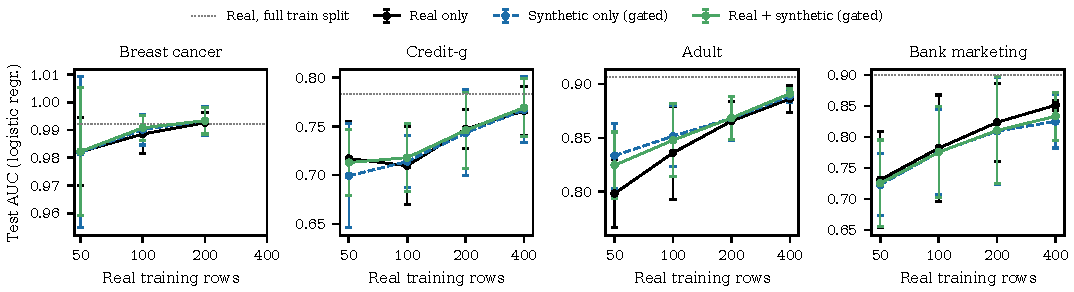
\includegraphics[width=\textwidth]{figures/scarcity.pdf}
\caption{Data scarcity (E2): test AUC of logistic regression trained on $n_{\mathrm{real}}$ real rows, on gated synthetic rows only (4 per real row), or on both. Mean and 95\% interval over five seeds. The dotted line is the model trained on the full train split.}
\label{fig:scarcity}
\end{figure*}

\subsubsection{Missing data}
Table~\ref{tab:missing} reports E3. Deleting 10\% or 30\% of numeric cells did not measurably change the utility ratio: every paired difference against the complete-data run had a 95\% interval that included zero (\texttt{missing\_effect.csv}). The rate-zero column is an independent replicate of the main experiment with different random streams, which is why it differs slightly from Table~\ref{tab:utility}. The TRTR baseline also degraded little, since HGB handles missing values natively and LR imputes medians. Only deletion completely at random was tested. Informative missingness was not.

% AUTO:BEGIN missing
\begin{table}[!t]
\caption{Utility ratio (HGB, mean over five seeds) when a fraction of numeric cells in the train and holdout splits is deleted completely at random. The breast-cancer set has no categorical columns; all others keep their categorical columns intact.}
\label{tab:missing}
\centering
\footnotesize
\setlength{\tabcolsep}{3pt}
\begin{tabular}{llrrr}
\toprule
Dataset & Condition & 0.0 & 0.1 & 0.3 \\
\midrule
Breast cancer & Copula, ungated & 1.002 & 0.996 & 0.999 \\
 & Orchestrated, gated & 0.999 & 0.999 & 0.998 \\
Credit-g & Copula, ungated & 0.975 & 0.956 & 0.996 \\
 & Orchestrated, gated & 0.968 & 0.961 & 0.997 \\
Adult & Copula, ungated & 0.988 & 0.986 & 0.988 \\
 & Orchestrated, gated & 0.986 & 0.985 & 0.988 \\
Bank marketing & Copula, ungated & 0.961 & 0.964 & 0.956 \\
 & Orchestrated, gated & 0.968 & 0.958 & 0.962 \\
\bottomrule
\end{tabular}
\end{table}
% AUTO:END missing

\subsubsection{Cost}
Table~\ref{tab:scaling} lists single-machine timings on Adult. Fitting took between 0.018 and 0.548 seconds, sampling 100000 rows took at most 0.228 seconds, and the gate evaluated a batch of 500 rows in 0.079 to 0.095 seconds. The privacy check is the scaling bottleneck. Computing the DCR share for 10000 synthetic rows took between 1.142 and 1.614 seconds, and the cost grows with the product of the synthetic and reference sizes. These timings come from one laptop. They do not support claims about cost reduction anywhere else.

% AUTO:BEGIN scaling
\begin{table}[!t]
\caption{Single-machine wall-clock seconds (median of three repetitions) on the Adult train split, seed 0. Fit uses the full train split; the other columns give the number of synthetic rows sampled or checked.}
\label{tab:scaling}
\centering
\footnotesize
\setlength{\tabcolsep}{2pt}
\begin{tabular}{lrrrrw{c}{27pt}w{c}{27pt}}
\toprule
 & & \multicolumn{3}{c}{Sample (rows)} & \multicolumn{2}{c}{DCR share (rows)} \\
Generator & Fit & 1000 & 10000 & 100000 & 1000 & 10000 \\
\midrule
Gaussian copula & 0.071 & 0.009 & 0.154 & 0.228 & 0.162 & 1.614 \\
Cl.-cond.\ GMM & 0.548 & 0.009 & 0.059 & 0.222 & 0.124 & 1.275 \\
SMOTE-style & 0.497 & 0.004 & 0.008 & 0.061 & 0.114 & 1.142 \\
Indep.\ marg. & 0.018 & 0.007 & 0.049 & 0.174 & 0.112 & 1.147 \\
\bottomrule
\end{tabular}
\end{table}
% AUTO:END scaling

\section{Threats to Validity}
\label{sec:threats}

\emph{Untested LLM layer.} No LLM was called. The rule-based planner exercises the gate, the fallback logic, and the outcome handling, but it says nothing about whether an LLM planner would choose better generators, explain rejections correctly, or bring new failure modes such as malformed configurations. Every result here applies to the rule-based pipeline only.

\emph{Unavailable baselines.} The CPU-only budget ruled out deep generators (CTGAN, TabDDPM, and LLM row generators such as GReaT) and differentially private generators (PrivBayes). They may reach higher fidelity, and some may memorise more. Our conclusions about the gate do not depend on the generator family. Our utility numbers do.

\emph{Construct validity.} The utility ratio uses ROC-AUC on one binary task per dataset and ignores calibration, subgroup error, and decision costs. Ratios above 1 occur because TSTR and TRTR are both noisy on small test splits. The attack is a distance-based lower bound on leakage; stronger attacks, such as shadow-model attacks, may succeed where ours fails. The DCR share and the attack use the same holdout that calibrates the gate, so the gated privacy numbers are not fully independent of the gate. The correlation distance works on frequency-ordered category codes, which put an arbitrary order on nominal columns.

\emph{Statistical validity.} Five seeds give wide intervals on the two small datasets. The primary hypothesis passed on credit-g with no margin and S1 passed narrowly on breast cancer, and we read both results as borderline. The secondary comparisons are reported without multiplicity correction.

\emph{Untested breakpoints.} Nothing beyond the 10000-row cap was tested, and fitting was not tried at much larger scale; only sampling was timed up to 100000 rows. Also untested: distribution shift between the real data and the deployment population, temporal drift, informative missingness, high-cardinality or free-text columns, multi-class or regression targets, and non-tabular data such as images and time series. Version~1 discussed several of these domains. None is supported here. Batch-level privacy checks were noisy for batches of about 50 rows or fewer. A pooled or sequential test would likely reduce both false rejections and missed copies, but we did not evaluate one.

\emph{Open questions.} Cost savings, development time, and regulatory compliance were not measured. Records that pass our gate can still disclose information about rare individuals, and passing the gate is not evidence of compliance with any regulation.

\section{Conclusion}
\label{sec:conclusion}
This revision replaced the unmeasured claims of version~1 with a preregistered benchmark. On four public tables, a gated pipeline of locally fitted generators retained between 96.1\% and 99.6\% of real-data test AUC, which supports the preregistered hypothesis of at least 90\% retention, with no margin on credit-g. The more useful finding is about what utility misses. Interpolating and copying generators kept near-real utility while a simple attack identified training members. A gate calibrated on real holdout data withheld those releases, and when a copier was placed first it lowered attack AUC to near chance. Its batch-level privacy test was noisy on small tables, which caused both false rejections and a few missed copies. Retry with fallback kept delivery high under simulated faults. Synthetic rows did not consistently improve models trained on small real samples. The LLM orchestration layer is still a design, and future work has to test it against the same gate and metrics.

\emph{Data and code availability.} The Zenodo package for this version contains the experiment code, the cached public datasets with their sources and checksums (\texttt{data/SOURCES.md}), all result files, the unit tests, the preregistration, and the \LaTeX{} source. Running \texttt{python code/run\_all.py} downloads or reuses the data, reruns every scenario with fixed seeds, and regenerates all tables and figures.

\section*{Acknowledgment}
This revision was prepared with generative AI. Large language models (GitHub Copilot with Anthropic Claude) critiqued the methodology, generated experiment code, drafted and edited the text, and in a last pass edited the wording. Every reported number, table, and figure was produced by code from logged experiment results; none was written by a language model.

\bibliographystyle{IEEEtran}
\bibliography{references}

\end{document}
